% Created 2022-03-27 dom 23:40
% Intended LaTeX compiler: pdflatex
\documentclass[11pt]{article}
\usepackage[utf8]{inputenc}
\usepackage[T1]{fontenc}
\usepackage{graphicx}
\usepackage{longtable}
\usepackage{wrapfig}
\usepackage{rotating}
\usepackage[normalem]{ulem}
\usepackage{amsmath}
\usepackage{amssymb}
\usepackage{capt-of}
\usepackage{hyperref}
\author{Diogo Garbinato de Fagundes}
\date{\today}
\title{Programa IT Academy - Processo Seletivo - Edição 15}
\hypersetup{
 pdfauthor={Diogo Garbinato de Fagundes},
 pdftitle={Programa IT Academy - Processo Seletivo - Edição 15},
 pdfkeywords={},
 pdfsubject={},
 pdfcreator={Emacs 27.2 (Org mode 9.6)}, 
 pdflang={English}}
\begin{document}

\maketitle
\tableofcontents


\section{Etapa}
\label{sec:org595af53}
\textbf{Enunciado:} Para ganhar a bolsa os candidatos precisam fazer algumas provas, são elas:
Conhecimento Gerais (CG), Conhecimento Específicos (CE), Português (P) e Matemática
(M). Cada prova tem a duração de 50 minutos e podem ser alocadas de hora em hora.
Devido ao número reduzido de fiscais:

\begin{itemize}
\item As provas serão num sábado, nos horários 8:00, 9:00, 10:00 e 11:00.
\item A prova de (CG) deve ser às 8:00.
\item A prova de (CE) deve ser após a prova de (P) e também após a prova de (CG).
\item As provas de (M) e (CE) devem ser em horários consecutivos, nessa ordem.
\end{itemize}

\subsection{Se a prova de CG for às 8:00, a prova de M deverá ser às:}
\label{sec:orgaa0fead}

(A) 9:00

(B) 10:00

(C) 11:00

\textbf{Resposta}: Letra B. Pois a prova de M deve ser diretamente antes da de CE, e a prova de CE tem que ser am algum momento depois da prova de P, logo, a prova de P deve ser às 9:00, a prova M às 10:00 e a prova CE às 11:00

\subsection{Se as provas CG e P forem respectivamente às 8:00 e 9:00, a prova de CE deve ser:}
\label{sec:org0bdc8b8}

(A) 10:00

(B) 8:00

(C) 11:00

(D) 9:00

\textbf{Resposta}: Letra C. Como mencionado anteriormente, a prova de CE deve ser obrigatoriamente consecutiva a prova de M, então, como os horários 8:00 e 9:00 já foram alocados, a prova de M tem que ser às 10:00, e a prova de CE às 11:00

\subsection{Qual das seguintes afirmações é necessariamente verdadeira}
\label{sec:orga8e4d7f}

(A) A prova P é após a prova de CE

(B) A prova M pode ser realizada antes da prova P

(C) A prova de CG é a primeira e a de CE é a última a ser realizada.

(D) Se mudar a prova de CG para 10:00 então a prova de M deve ser as 8:00

\textbf{Resposta}: Letra C. Devido às regras dadas nos pontos levantados no enunciado, chegamos a uma ordem absoluta de como devem ser realizadas as provas. Começamos pela prova CG pois uma das regras é que a prova de CG deve ser às 8:00, e esse é o primeiro horário disponível, logo, é a primeira prova a ser realizada, assim como a alternativa C diz. Sabemos que a prova CE deve ser após a prova P e após a prova M por causa do terceiro e quarto pontos levantados no enunciado. Logo a prova de CE só pode ser a última a ser realizada, tornando a alternativa C necessariamente verdadeira.

\section{Etapa}
\label{sec:orgc6716c9}
Na resolução da segunda etapa eu escolhi utilizar a linguagem de programação C, e o console como interface. É importante ressaltar que este programa foi desenvolvido em um sistema operacional Linux, e consequentemente tentar compilar e executar o programa em outro sistema operacional como Windows ou macOS poderá gerar resultados diferentes.

Para desenvolver este programa eu comecei criando uma variável global que irá armazenar todo o arquivo .csv em um array bi-dimensional. Assim facilitando a manipulação dos dados, e tendo que abrir o arquivo para leitura apenas uma vez. Como C não possuí Strings, utilizei um array de char bi-dimensional, sendo: [linha][caracter].

O método main abre o arquivo e caso tenha sucedido em encontra o arquivo, lê e salva cada caracter do arquivo no array, através de dois do\ldots{}while. Depois ele entra no ``menu'' onde imprime na tela as opções de funções e utiliza um switch/case para ver qual função o usuário escolheu.

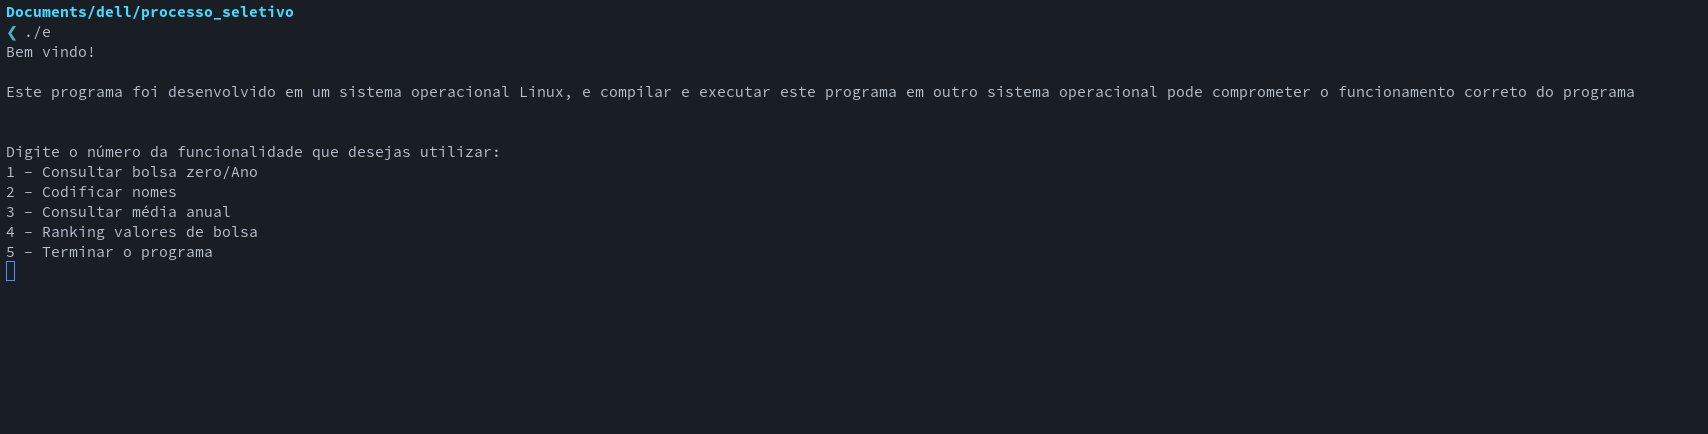
\includegraphics[width=15cm]{menu.png}

\subsection{Primeira funcionalidade}
\label{sec:org953db16}
Para solucionar a primeira funcionalidade eu criei um método auxiliar, que será reutilizado em outras funcionalidades também, o método \emph{``procuraAno''}, ele recebe um inteiro e um \emph{array} de \emph{char} por parâmetro. O inteiro é a linha do arquivo que queremos começar a procurar o ano, isso será útil na terceira funcionalidade. O \emph{array} de \emph{char} é o ano que o usuário quer consultar. O método retorna um inteiro, que será a linha do arquivo onde se encontra o ano, ou 0 no caso de não encontrar o ano.

Esse método usa um laço do tipo \emph{while} que se encerra caso termine o arquivo, ou encontre o ano que está sendo procurado. O arquivo .csv no formato de texto utiliza \emph{';'} para separar as células (ou categorias) na linha, então para encontrar o ano eu utilizei um loop que vai lendo caracter por caracter a linha até encontrar o quarto \emph{';'} (no código se vê o número 59, pois esse é o número do ';' na tabela ASCII), pois após ele, os dígitos que vem são o ano de referência. Após encontrar o ano na linha, eu utilizo um \emph{for} que compara os caracteres do ano na linha e o ano inserido pelo usuário. Cada vez que o laço encontra um caracter igual ele adiciona em um somatório; se no final do laço o somatório for 4 significa que todos os caracteres são iguais, ou seja, é o ano procurado. Daí o programa salva a linha do arquivo onde se encontra o ano desejado e retorna o método.

Depois de encontrar (ou não) o ano desejado, se imprime os dados do ``bolsista zero'' através de outro método auxiliar chamado imprimeCaracteres. Esse método recebe dois inteiros, que seriam, a linha e o local da linha para começar a imprimir. Ele imprime na tela caracter por caracter até encontrar o próximo ';', ou o fim da linha, depois retorna o local da linha onde estava (o caractere após ';'), para assim poder continuar indo seção por seção desejada das informações solicitadas no exercício.

Os três primeiros dados são consecutivos, então eu basicamente só chamo esse método auxiliar 3 vezes seguidas. Depois precisamos imprimir o valor da bolsa, que fica 7 células a frente da última que mostramos na tela (entidade de ensino), por isso utilizei um while que percorre a linha até encontrar mais 6 ';', depois mostro na tela qual é a moeda, pulo o ';', e mostro o número do valor da bolsa.

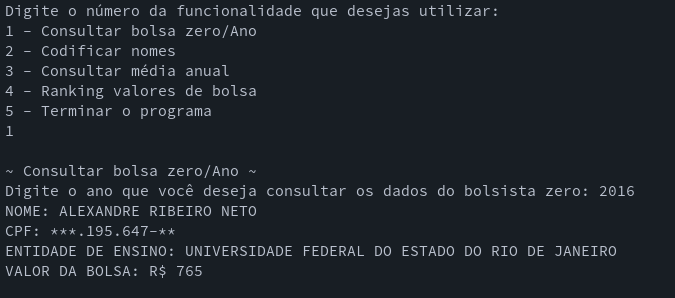
\includegraphics[width=10cm]{func1.png}

\subsection{Segunda funcionalidade}
\label{sec:org5958951}
Para desenvolver a segunda funcionalidade do programa eu primeiro analisei o padrão de codificação que foi utilizado nos exemplos do enunciado. Cheguei a conclusão de que primeiro devemos inverter todos os caracteres, menos o primeiro e o último, depois devemos trocar a letra pela próxima do alfabeto, e caso a letra seja Z (última do alfabeto) devemos trocar pela primeira letra, a letra A.

Eu começo o método da funcionalidade criando um array de char para armazenar o nome que o usuário deseja procurar e utilizei o \emph{fgets} para ler o input do usuário, pois essa função lê o input até uma quebra de linha, diferentemente do \emph{scanf}, que ao ter um espaço irá parar de ler o input. Depois criei mais um método auxiliar chamado '\emph{procuraUauraio}', que recebe o nome digitado por parâmetro. A lógica por trás desse método é similar a do '\emph{procuraAno}', a diferença é que o nome do usuário sempre começa na posição 0 do array do arquivo, assim não sendo necessário esse contador.

Depois, se o nome tiver sido encontrado no arquivo passamos para outro método auxiliar chamado '\emph{codificaNome}', que recebe por parâmetro a linha onde se encontra o bolsista. Primeiro eu armazeno o nome do bolsista em dois arrays de char, o primeiro é para referência, e o segundo será modificado para codificar o nome. Depois, utilizo um \emph{for} com o tamanho do nome, e vou trocando cada letra com a sua letra espelhada (por exemplo primeira letra troca com a última letra, segunda letra com a penúltima e assim por diante).

Depois uso mais um for, que pega caracter por caracter e substituí pelo próximo do alfabeto (utilizando a tabela ASCII é somar 1), mas antes verificar se o caracter não é um espaço em branco ou uma letra Z, se for a letra Z substituo por A, e se for espaço em branco não faço nada. Por fim imprime na tela o nome codificado. Depois imprimo os outros dados do bolsista requeridos no exercício, utilizando a mesma lógica da primeira funcionalidade.

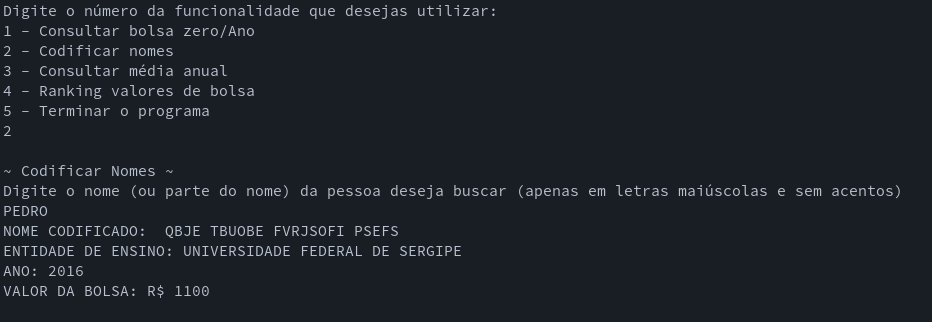
\includegraphics[width=10cm]{func2.png}

\subsection{Terceira funcionalidade}
\label{sec:orga96aa12}
Para a terceira funcionalidade é utilizado o método auxiliar '\emph{procuraAno}' já explicado na primeira funcionalidade. Caso encontre o ano, entra em um loop \emph{while} até não serem encontrados dados no ano desejado (assim o método auxiliar retornará 0). Nesse loop é utilizado um contador, que cada vez que encontra o ano, soma 1, além disso utilizo uma variável somatória, que toda vez que é encontrado o ano, soma o valor da bolsa com o próprio somatório. Depois de terminar o loop divido o somatório total pela quantidade de vezes que o ano foi encontrado, assim obtendo a média de bolsa daquele ano.

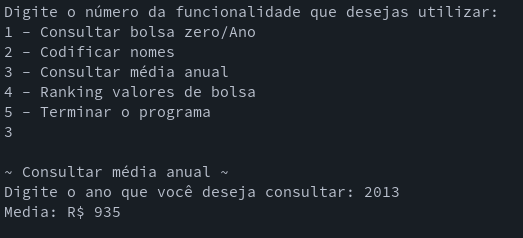
\includegraphics[width=10cm]{func3.png}

\subsection{Quarta funcionalidade}
\label{sec:orgfca00f7}
Para desenvolver a quarta funcionalidade eu criei um array bidimensional de inteiros, no tamanho 6x2, os 3 primeiros (dos 6) são os 3 bolsistas com as maiores bolsas, será armazenado a linha do bolsista e o valor de sua bolsa. Os últimos 3 são os bolsistas com as menores bolsas.
Primeiro eu coloco o valor de 0 no array das maiores bolsas, assim qualquer bolsista terá uma bolsa maior, e coloco um valor absurdamente alto no das menores bolsas, assim qualquer aluno terá uma bolsa menor.
Eu criei outro método auxiliar chamado '\emph{valorBolsa}' que recebe por parâmetro a linha do bolsista que queremos saber a bolsa. O método, primeiro encontra o décimo ';' pois depois dele se encontram os números do valor da bolsa. Como não é fixo a quantidade de caracteres que a bolsa vai ter (algumas bolsas são 3 outras são 4), tive que desenvolver uma lógica para a conversão de char para int, onde não precisamos saber a quantidade de digitos previamente. Basicamente, ele armazena o digito em uma variavel, e se não for o ultimo digito da linha, multiplica por 10, assim sempre tendo as casas decimais corretamente quando somarmos com o próximo digito (por exemplo: 1500 -> 1 * 10 = 10; 10 + 5 = 15; 15 * 10 = 150; 150 + 0 = 150 * 10 = 1500; 1500 + 0 = 1500). Por fim, o método retorna o valor da bolsa em inteiro.

A lógica para encontrar os alunos com maiores e menores bolsas é bem simples; ele compara a bolsa do bolsista atual com as bolsas dos bolsistas já armazenados no array 1 por 1, se for maior do que algum dos 3 primeiros troca, trocando os outros também que vem depois (caso não seja o terceiro mais baixo ou terceiro mais alto).

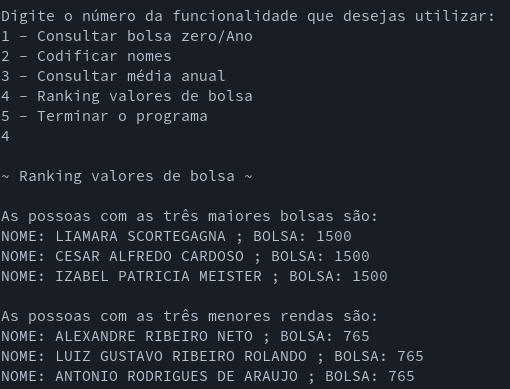
\includegraphics[width=10cm]{func4.png}

\subsection{Quinta funcionalidade}
\label{sec:orgf4eaff4}
Eu fiz o menu principal um loop do tipo \emph{while}, e o programa só encerra quando o usuário enviar o número 5, assim permitindo que ele encerre o programa.

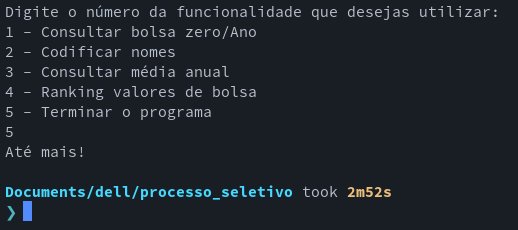
\includegraphics[width=10cm]{func5.png}

\section{Autoavaliação}
\label{sec:org65b4597}

Achei o exercício, tanto a etapa 1 quanto a etapa 2 relativamente fácil e divertido, a etapa 1 consegui realizar sem nenhuma dificuldade. Já na etapa dois eu tive uma dificuldade maior para começar a desenvolver o programa, mas quando eu tive a ideia de armazenar o arquivo inteiro em um array bi-dimensional tive mais facilidade em pensar nas soluções das funcionalidades. Tive que me esforçar bastante para desenvolver a primeira funcionalidade, mas após essa, todas as outras seguem a mesma lógica, então só tive que adaptar para cada particularidade de cada funcionalidade. Para testes, realizei testes com diversas entradas de dados, tanto dados válidos quanto inválidos e chequei se estavam de acordo com o documento .csv
\end{document}
